
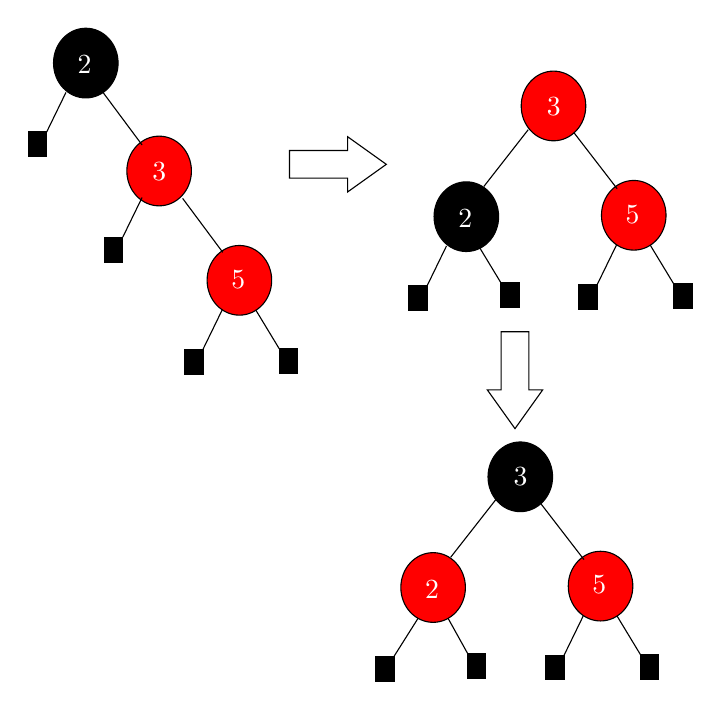
\begin{tikzpicture}[x=0.5pt,y=0.5pt,yscale=-1,xscale=1]
%uncomment if require: \path (0,706); %set diagram left start at 0, and has height of 706

\draw  [fill={rgb, 255:red, 0; green, 0; blue, 0 }  ,fill opacity=1 ]  (20.22, 217.65) rectangle (33.54, 235.61)   ;
\draw    (33.54,217.65) -- (47.5,189) ;


\draw  [fill={rgb, 255:red, 0; green, 0; blue, 0 }  ,fill opacity=1 ]  (61.83, 167.82) circle [x radius= 23.33, y radius= 25.18]  ;
\draw    (184.5,346) -- (201.62,374.26) ;


\draw  [fill={rgb, 255:red, 0; green, 0; blue, 0 }  ,fill opacity=1 ]  (201.62, 374.26) rectangle (214.94, 392.22)   ;
\draw  [fill={rgb, 255:red, 255; green, 0; blue, 0 }  ,fill opacity=1 ]  (114.83, 245.82) circle [x radius= 23.33, y radius= 25.18]  ;
\draw    (73.5,188) -- (102.5,227) ;


\draw  [fill={rgb, 255:red, 0; green, 0; blue, 0 }  ,fill opacity=1 ]  (75.22, 293.65) rectangle (88.54, 311.61)   ;
\draw    (88.54,293.65) -- (102.5,265) ;


\draw  [fill={rgb, 255:red, 255; green, 0; blue, 0 }  ,fill opacity=1 ]  (172.83, 324.82) circle [x radius= 23.33, y radius= 25.18]  ;
\draw    (131.83,265.64) -- (160.83,304.64) ;


\draw  [fill={rgb, 255:red, 0; green, 0; blue, 0 }  ,fill opacity=1 ]  (133.22, 374.65) rectangle (146.54, 392.61)   ;
\draw    (146.54,374.65) -- (160.5,346) ;


\draw   (209,231) -- (251,231) -- (251,221) -- (279,241) -- (251,261) -- (251,251) -- (209,251) -- cycle ;
\draw  [fill={rgb, 255:red, 0; green, 0; blue, 0 }  ,fill opacity=1 ]  (295.22, 328.65) rectangle (308.54, 346.61)   ;
\draw    (308.54,328.65) -- (322.5,300) ;


\draw  [fill={rgb, 255:red, 0; green, 0; blue, 0 }  ,fill opacity=1 ]  (336.83, 278.82) circle [x radius= 23.33, y radius= 25.18]  ;
\draw    (469.5,299) -- (486.62,327.26) ;


\draw  [fill={rgb, 255:red, 0; green, 0; blue, 0 }  ,fill opacity=1 ]  (486.62, 327.26) rectangle (499.94, 345.22)   ;
\draw  [fill={rgb, 255:red, 255; green, 0; blue, 0 }  ,fill opacity=1 ]  (399.83, 198.82) circle [x radius= 23.33, y radius= 25.18]  ;
\draw  [fill={rgb, 255:red, 255; green, 0; blue, 0 }  ,fill opacity=1 ]  (457.83, 277.82) circle [x radius= 23.33, y radius= 25.18]  ;
\draw    (414.5,218) -- (445.83,258.64) ;


\draw  [fill={rgb, 255:red, 0; green, 0; blue, 0 }  ,fill opacity=1 ]  (418.22, 327.65) rectangle (431.54, 345.61)   ;
\draw    (431.54,327.65) -- (445.5,299) ;


\draw    (349.5,257) -- (381.6,215.92) ;


\draw    (344.5,298) -- (361.62,326.26) ;


\draw  [fill={rgb, 255:red, 0; green, 0; blue, 0 }  ,fill opacity=1 ]  (361.62, 326.26) rectangle (374.94, 344.22)   ;
\draw   (382,362) -- (382,404) -- (392,404) -- (372,432) -- (352,404) -- (362,404) -- (362,362) -- cycle ;
\draw  [fill={rgb, 255:red, 0; green, 0; blue, 0 }  ,fill opacity=1 ]  (271.22, 596.65) rectangle (284.54, 614.61)   ;
\draw    (284.54,596.65) -- (302,569) ;


\draw  [fill={rgb, 255:red, 255; green, 0; blue, 0 }  ,fill opacity=1 ]  (312.83, 546.82) circle [x radius= 23.33, y radius= 25.18]  ;
\draw    (445.5,567) -- (462.62,595.26) ;


\draw  [fill={rgb, 255:red, 0; green, 0; blue, 0 }  ,fill opacity=1 ]  (462.62, 595.26) rectangle (475.94, 613.22)   ;
\draw  [fill={rgb, 255:red, 0; green, 0; blue, 0 }  ,fill opacity=1 ]  (375.83, 466.82) circle [x radius= 23.33, y radius= 25.18]  ;
\draw  [fill={rgb, 255:red, 255; green, 0; blue, 0 }  ,fill opacity=1 ]  (433.83, 545.82) circle [x radius= 23.33, y radius= 25.18]  ;
\draw    (390.5,486) -- (421.83,526.64) ;


\draw  [fill={rgb, 255:red, 0; green, 0; blue, 0 }  ,fill opacity=1 ]  (394.22, 595.65) rectangle (407.54, 613.61)   ;
\draw    (407.54,595.65) -- (421.5,567) ;


\draw    (325.5,525) -- (358.6,482.74) ;


\draw    (323.6,569.01) -- (337.62,594.26) ;


\draw  [fill={rgb, 255:red, 0; green, 0; blue, 0 }  ,fill opacity=1 ]  (337.62, 594.26) rectangle (350.94, 612.22)   ;

\draw (61,169) node [color={rgb, 255:red, 255; green, 255; blue, 255 }  ,opacity=1 ] [align=left] {2};
\draw (115,246) node [color={rgb, 255:red, 255; green, 255; blue, 255 }  ,opacity=1 ] [align=left] {3};
\draw (172,324) node [color={rgb, 255:red, 255; green, 255; blue, 255 }  ,opacity=1 ] [align=left] {5};
\draw (336,280) node [color={rgb, 255:red, 255; green, 255; blue, 255 }  ,opacity=1 ] [align=left] {2};
\draw (400,199) node [color={rgb, 255:red, 255; green, 255; blue, 255 }  ,opacity=1 ] [align=left] {3};
\draw (457,277) node [color={rgb, 255:red, 255; green, 255; blue, 255 }  ,opacity=1 ] [align=left] {5};
\draw (312,548) node [color={rgb, 255:red, 255; green, 255; blue, 255 }  ,opacity=1 ] [align=left] {2};
\draw (376,467) node [color={rgb, 255:red, 255; green, 255; blue, 255 }  ,opacity=1 ] [align=left] {3};
\draw (433,545) node [color={rgb, 255:red, 255; green, 255; blue, 255 }  ,opacity=1 ] [align=left] {5};


\end{tikzpicture}